\section{Instalacja i konfiguracja środowiska}
\label{sec:instalacja}

\subsection{Anaconda}
\label{sec:anaconda}

Instalację rozpoczynamy od interpretera Anaconda. Pliki instalacyjne pobrać można z oficjalnej strony Anacondy \hyperref[anaconda]{''https://anaconda.org/anaconda/python ''}. Na stronie powinniśmy znaleźć pliki instalacyjne dla różnych systemów operacyjnych. Pobieramy plik odpowiedni dla naszego systemu. W omawianym przypadku będzie to win-64. Pliki instalacyjne zawarte są na płycie CD dołączonej do pracy.

Po zainstalowaniu Anacondy należy dodać jej ścieżkę do zmiennych systemowych. W tym celu wymagane są uprawnienie administratora. Poniżej znajdują się instrukcja dodawania ścieżki oraz sposób sprawdzenia czy Anaconda jest widoczna przez system.

Otwieramy ,,Panel Sterowania'' (,,Control Panel''). Wchodzimy w zakładkę ,,System i Zabezpieczenia'' (,,System and Security''), rysunek \ref{fig:anaconda1}, a następnie w ,,System'', rysunek \ref{fig:anaconda2}. Z lewej strony klikamy ,,Zaawansowane ustawienia systemu'' (,,Advanced system settings''), rysunek \ref{fig:anaconda3}, a następnie
,,Zmienne środowiskowe'' (,,Environment variables''), rysunek \ref{fig:anaconda4}. Znajdujemy zmienną ,,Ścieżka'' (,,Path''), rysunek \ref{fig:anaconda5} i otwieramy ją przez dwukrotne kliknięcie myszką. Przesuwamy do końca tekst w nowo otwartym oknie i dopisujemy na końcu średnik, ścieżkę do folderu gdzie zainstalowaliśmy Anacondę, kolejny średnik i ścieżkę do folderu Scripts, który znajduje się w katalogu Anacondy, rysunek \ref{fig:anaconda6}. Przykładowe ścieżki to ;F:\textbackslash Programy\textbackslash Anaconda;F:\textbackslash Programy\textbackslash Anaconda\textbackslash Scripts. We wszystkich oknach które otworzyliśmy klikamy OK.

Aby sprawdzić czy całość operacji przebiegła pomyślnie należy otworzyć ,,Wiersz Poleceń'' (,,Command Prompt''), np. poprzez kliknięcie symbulu Windows na klawiaturze, wpisanie ,,cmd'' i otwarcie znalezionej aplikacji.W otwartym oknie wpisujemy komendę ,,conda'', rysunek \ref{fig:anaconda7}.  Jeśli jest ona rozpoznana to dostaniemy odpowiedź jak na rysunku \ref{fig:anaconda8}. Jeśli komenda nie zostanie rozpoznana, należy sprawdzic poprzednie kroki oraz prawidłowość ścieżek dodanych do zmiennej ,,Path''.

\begin{figure}[h]
\centering
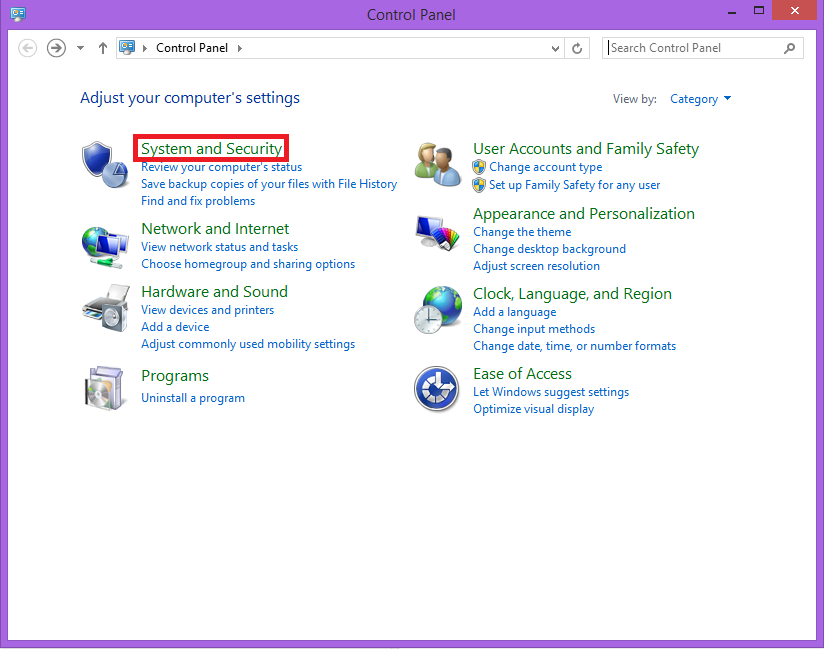
\includegraphics[width=10cm]{Zdjecia/5/anaconda1}
\caption{Widok panelu sterowania}
\label{fig:anaconda1}
\end{figure}

\begin{figure}[h]
\centering
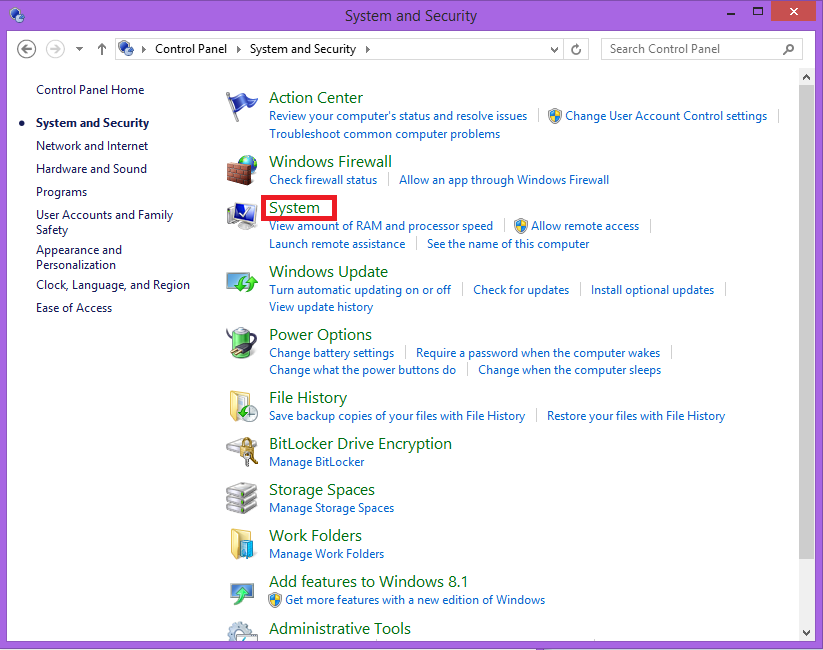
\includegraphics[width=10cm]{Zdjecia/5/anaconda2}
\caption{Zakłada System i Zabezpieczenia}
\label{fig:anaconda2}
\end{figure}

\begin{figure}[h]
\centering
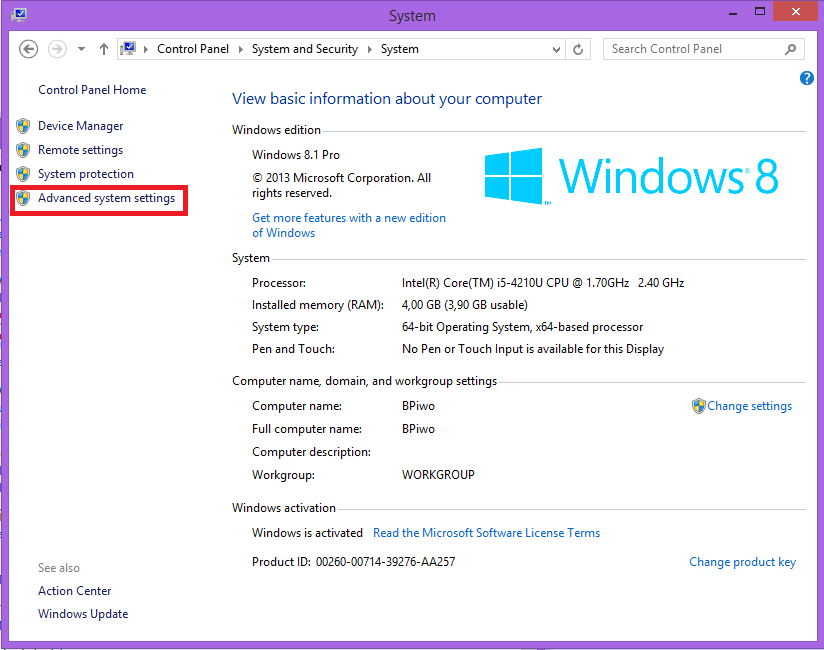
\includegraphics[width=10cm]{Zdjecia/5/anaconda3}
\caption{Zakładka System}
\label{fig:anaconda3}
\end{figure}

\begin{figure}[h]
\centering
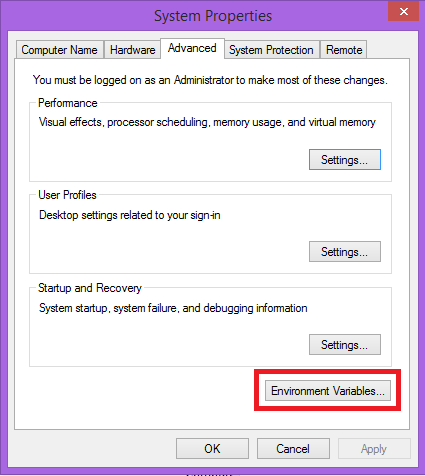
\includegraphics[width=10cm]{Zdjecia/5/anaconda4}
\caption{Okno Zaawansowane ustawienia systemu}
\label{fig:anaconda4}
\end{figure}

\begin{figure}[h]
\centering
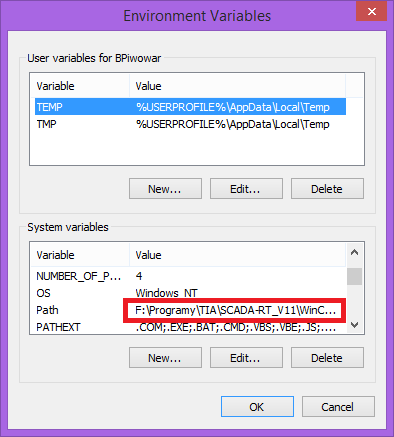
\includegraphics[width=10cm]{Zdjecia/5/anaconda5}
\caption{Okno Zmienne środowiskowe}
\label{fig:anaconda5}
\end{figure}

\begin{figure}[h]
\centering
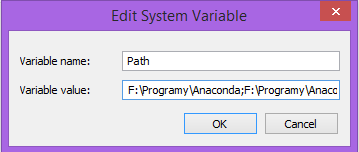
\includegraphics[width=10cm]{Zdjecia/5/anaconda6}
\caption{Okno zmiennej Path}
\label{fig:anaconda6}
\end{figure}


\begin{figure}[h]
\centering
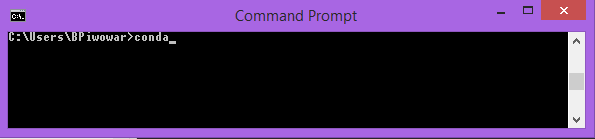
\includegraphics[width=10cm]{Zdjecia/5/anaconda7}
\caption{Wiersz Poleceń}
\label{fig:anaconda7}
\end{figure}

\begin{figure}[h]
\centering
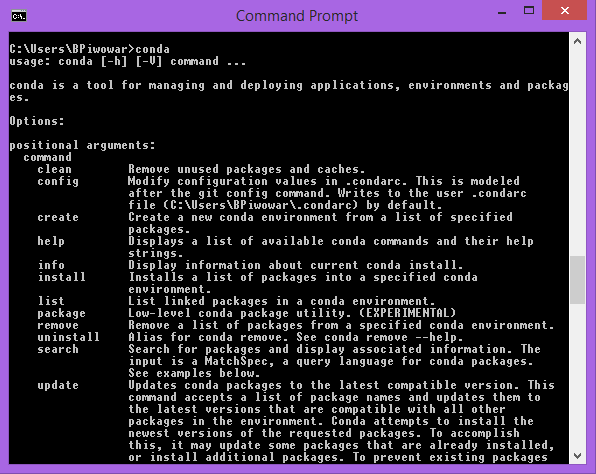
\includegraphics[width=10cm]{Zdjecia/5/anaconda8}
\caption{Odpowiedź na komendę ,,Conda''}
\label{fig:anaconda8}
\end{figure}

\subsection{PyCharm}
\label{sec:pycharm}

IDE wykorzystywanym w projekcie jest PyCharm. Program jest dostępny do pobrania pod linkiem https:\textbackslash \textbackslash www.jetbrains.com\textbackslash pycharm\textbackslash download\textbackslash \#section=windows. Dodatkowo plik instalacyjny jest zamieszczony na płycie CD dołączonej do pracy. Po zainstalowaniu programu, można otworzyć projekt aplikacji w standardowy sposób tj. File -> Open. W oknie, które się otworzy należy wskazać katalog projektu.

Ostatnia rzecz dotycząca konfiguracji to ustawienie aktywnego interpretera dla projektu. W tym celu wchodzimy należy wejść w ustawienia (,,Settings''), rysunek \ref{fig:pycharm1}. Następnie otwieramy zakładkę ,,Project'', klikamy na ,,Project interpreter'' i w pasku wyboru na górze wybieramy interpreter ze ścieżką, gdzie zainstalowaliśmy Anacondę, rysunek \ref{fig:pycharm2}.

\begin{figure}[h]
\centering
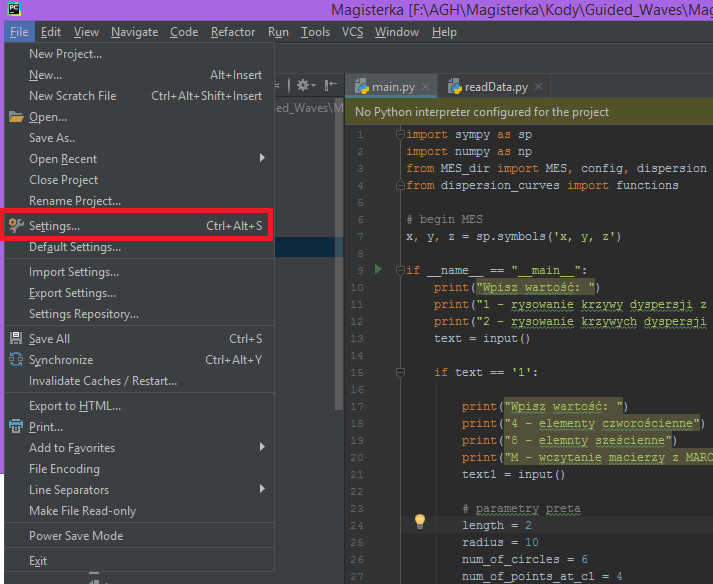
\includegraphics[width=10cm]{Zdjecia/5/pycharm1}
\caption{Okno główne projektu w programie PyCharm}
\label{fig:pycharm1}
\end{figure}

\begin{figure}[h]
\centering
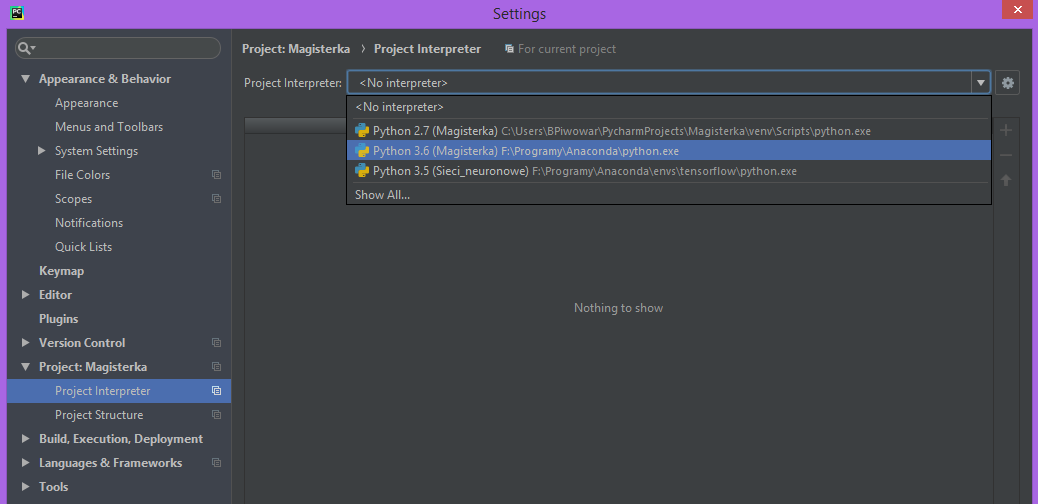
\includegraphics[width=10cm]{Zdjecia/5/pycharm2}
\caption{Wybór interpretera}
\label{fig:pycharm2}
\end{figure}










